\addcontentsline{toc}{subsection}{Inciso h}

\subsection*{h.}

\textbf{A lo largo del tiempo han existido diversos modelos de datos, como el modelo jerárquico, el modelo de red, el modelo relacional, el modelo orientado a objetos y los modelos NoSQL (llave-valor, documento, columnares, grafos).Responde lo siguiente:}

 \noindent \textbf{Elabora una tabla comparativa entre al menos cuatro modelos de datos, destacando sus principales características, ventajas, desventajas y casos de uso típicos.}
\begin{figure}[H]
    \makebox[\textwidth][c]{%
        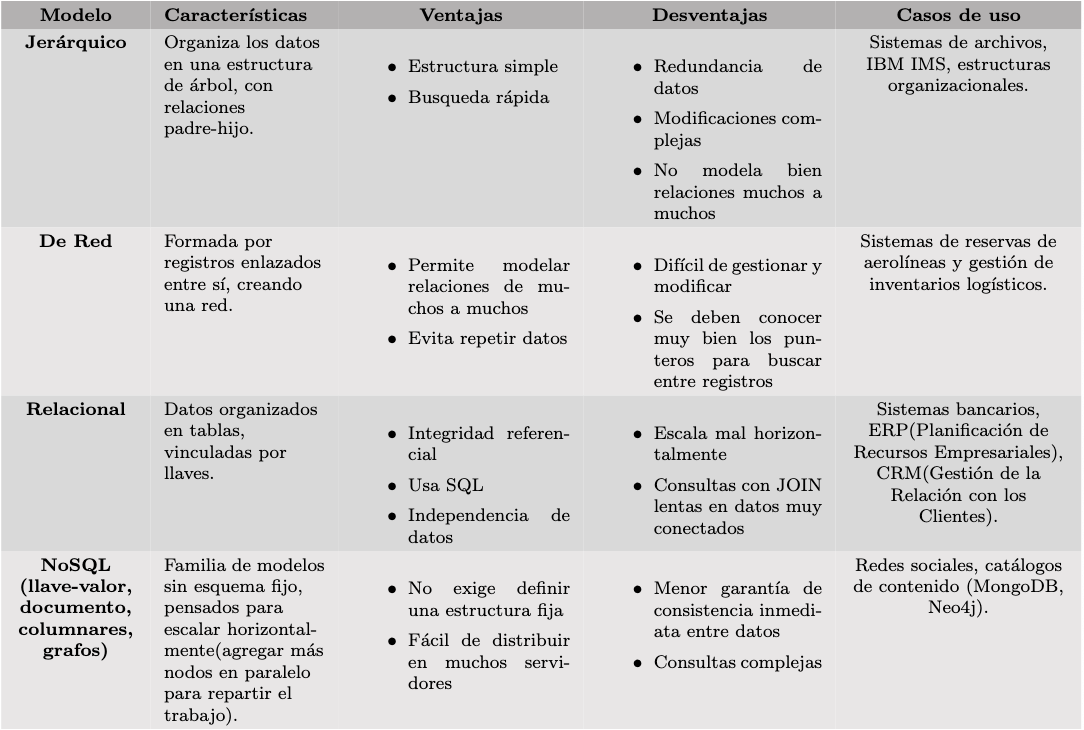
\includegraphics[width=1.2\linewidth]{imagenes/TABLA.png}%
    }
\end{figure}
\noindent \textbf{¿Por qué crees que el modelo relacional se convirtió en el más ampliamente adoption durante décadas?}

Al estar basado en la teoría de conjuntos y álgebra relacional, proporcionó una fomra estructurada de representar las relaciones entre los datos.

Ádemas, la creación de SQL como lenguaje estándar facilitó la formación de profesionales, estableciendo una forma común de trabajar con las bases de datos.

Por último, al permitir forzar la integridad y consistencia de los datos de forma declarativa, generó una gran confianza para su uso en aplicaciones empresariales, como sistemas bancarios y de comercio, que contribuyó a consolidarlo como el modelo dominante por décadas.

\textbf{¿En qué contextos actuales los modelos NoSQL superan al modelo relacional en eficiencia o flexibilidad? Justifica con ejemplos.}

Las bases de datos NoSQL ofrecen mayor rendimiento y adaptabilidad cuando se trabaja con grandes volúmenes de datos no estructurados.

Los principales contextos donde los modelos NoSQL destacan son:
\begin{itemize}
    \item Cuando existen grandes volúmenes de datos distribuidos con escrituras de alta frecuencia.
    \item Al manejar datos semiestructurados o no estructurados, como catálogos con atributos variables, bitácoras y eventos.
    \item En aplicaciones que requieren rapidez de respuesta en lecturas simples, como sesiones de usuario, caché o contadores.
    \item En entornos IoT, donde se presentan ingestas masivas de datos provenientes de múltiples dispositivos.
    \item En redes sociales, catálogos de productos y sistemas de recomendación con esquemas cambiantes.
    \item Durante procesos de analítica distribuida donde los datos se procesan en múltiples nodos.
    \item En proyectos donde el esquema evoluciona con frecuencia.
\end{itemize}
